\paragraph{CSE572 Statistical Machine Learning - Project 1 - Density Estimation and Classification Project}

\subparagraph{Import Libraries}

\begin{verbatim}
import math
import numpy as np
import pandas as pd

import matplotlib.pyplot as plt

import scipy.io
from scipy.stats import norm

from sklearn.metrics import confusion_matrix, accuracy_score
import seaborn as sns
\end{verbatim}

\subparagraph{Process Image Files into Data Objects}

\begin{verbatim}
myID='5806' #change to last 4 digit of your studentID
geneNewData.geneData(myID)
Numpyfile0 = scipy.io.loadmat('digit0_stu_train'+myID+'.mat')
Numpyfile1 = scipy.io.loadmat('digit1_stu_train'+myID+'.mat')
Numpyfile2 = scipy.io.loadmat('digit0_testset'+'.mat')
Numpyfile3 = scipy.io.loadmat('digit1_testset'+'.mat')
train0 = Numpyfile0.get('target_img')
train1 = Numpyfile1.get('target_img')
test0 = Numpyfile2.get('target_img')
test1 = Numpyfile3.get('target_img')
print([len(train0),len(train1),len(test0),len(test1)])
print('Your trainset and testset are generated successfully!')
\end{verbatim}

\begin{verbatim}
[5000, 5000, 980, 1135]
Your trainset and testset are generated successfully!
\end{verbatim}

\subparagraph{Exploratory Data Analysis}

\subparagraph{Obtain Dimensions of Given Image Data Objects}

\begin{verbatim}
train0.shape
\end{verbatim}

\begin{verbatim}
(5000, 28, 28)
\end{verbatim}

\begin{verbatim}
train0[0].max()
\end{verbatim}

\begin{verbatim}
255
\end{verbatim}

\begin{verbatim}
train0[0].min()
\end{verbatim}

\begin{verbatim}
0
\end{verbatim}

\begin{verbatim}
train1.shape
\end{verbatim}

\begin{verbatim}
(5000, 28, 28)
\end{verbatim}

\begin{verbatim}
test0.shape
\end{verbatim}

\begin{verbatim}
(980, 28, 28)
\end{verbatim}

\begin{verbatim}
test1.shape
\end{verbatim}

\begin{verbatim}
(1135, 28, 28)
\end{verbatim}

\subparagraph{Visualize First Train 0 Image}

\begin{verbatim}
ticks = np.arange(0, 28+2, 2)
ticks
\end{verbatim}

\begin{verbatim}
array([ 0,  2,  4,  6,  8, 10, 12, 14, 16, 18, 20, 22, 24, 26, 28])
\end{verbatim}

\begin{verbatim}
plt.imshow(train0[1], cmap='grey')
plt.xlim(0, 28)
plt.xticks(ticks=ticks)
plt.yticks(ticks=ticks)
plt.show()
\end{verbatim}

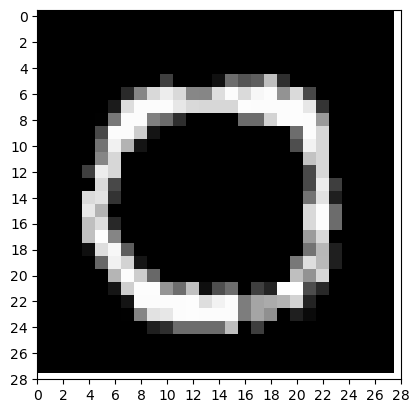
\includegraphics[width=0.7\linewidth]{files/44da2711dc53cb1cc59948168c0757dc.png}

\subparagraph{Visualize the First 10 Train0 Images}

\begin{verbatim}
# Display the first 10 images
num_images_to_display = 10
plt.figure(figsize=(10, 5))  # Adjust the figure size

for i in range(num_images_to_display):
    plt.subplot(2, 5, i + 1)  # Create a 2x5 grid for 10 images
    plt.imshow(train0[i], cmap='gray')  # Display each image
    plt.title(f'Train0 Image {i + 1}')
    plt.axis('off')  # Hide axes for better visualization

plt.tight_layout()
plt.show()
\end{verbatim}

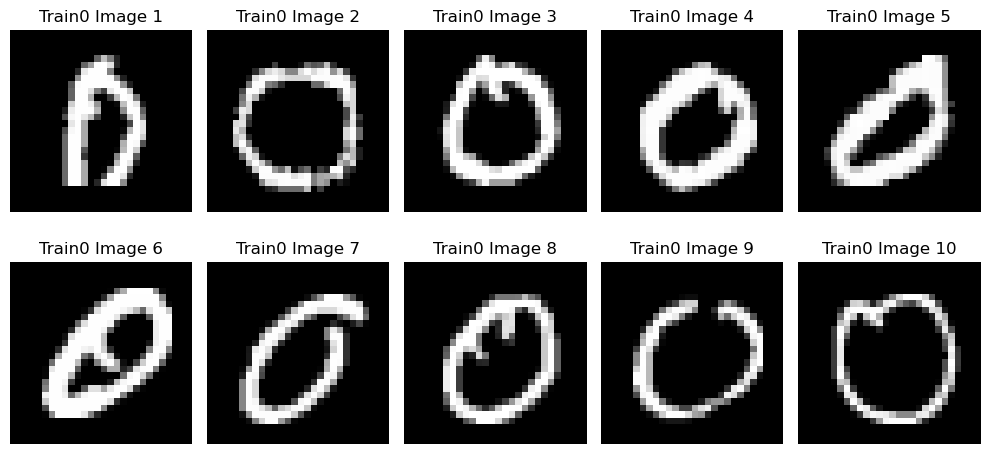
\includegraphics[width=0.7\linewidth]{files/64dc240e272cab33efbd930a21cbfe53.png}

\subparagraph{Visualize the First 10 Train1 Images}

\begin{verbatim}
# Display the first 10 images
num_images_to_display = 10
plt.figure(figsize=(10, 5))  # Adjust the figure size

for i in range(num_images_to_display):
    plt.subplot(2, 5, i + 1)  # Create a 2x5 grid for 10 images
    plt.imshow(train1[i], cmap='gray')  # Display each image
    plt.title(f'Train1 Image {i + 1}')
    plt.axis('off')  # Hide axes for better visualization

plt.tight_layout()
plt.show()
\end{verbatim}

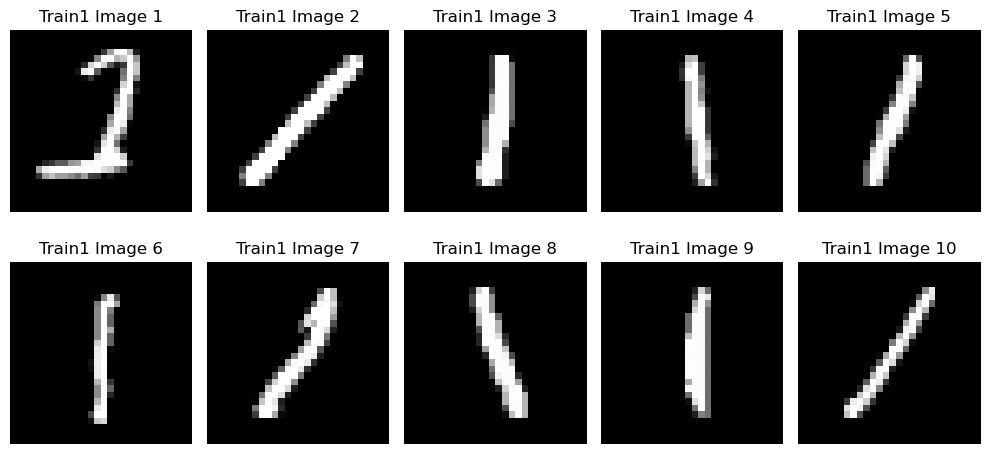
\includegraphics[width=0.7\linewidth]{files/e5505aac11d3d9c9ad7344db9b42a083.png}

\subparagraph{Visualize the First 10 Test0 Images}

\begin{verbatim}
# Display the first 10 images
num_images_to_display = 10
plt.figure(figsize=(10, 5))  # Adjust the figure size

for i in range(num_images_to_display):
    plt.subplot(2, 5, i + 1)  # Create a 2x5 grid for 10 images
    plt.imshow(test0[i], cmap='gray')  # Display each image
    plt.title(f'Test0 Image {i + 1}')
    plt.axis('off')  # Hide axes for better visualization

plt.tight_layout()
plt.show()
\end{verbatim}

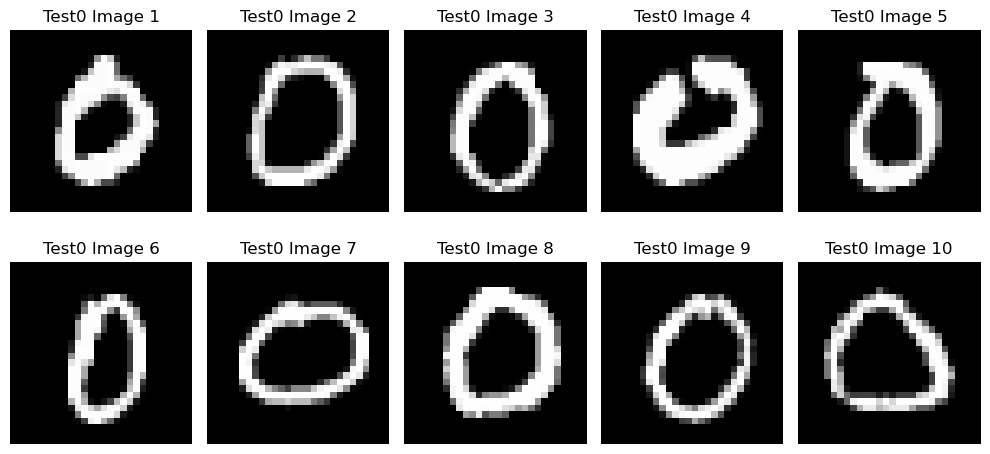
\includegraphics[width=0.7\linewidth]{files/8a453c2f8e1ecdd657cc62bc8494b5dd.png}

\subparagraph{Visualize the First 10 Test1 Images}

\begin{verbatim}
# Display the first 10 images
num_images_to_display = 10
plt.figure(figsize=(10, 5))  # Adjust the figure size

for i in range(num_images_to_display):
    plt.subplot(2, 5, i + 1)  # Create a 2x5 grid for 10 images
    plt.imshow(test1[i], cmap='gray')  # Display each image
    plt.title(f'Test0 Image {i + 1}')
    plt.axis('off')  # Hide axes for better visualization

plt.tight_layout()
plt.show()
\end{verbatim}

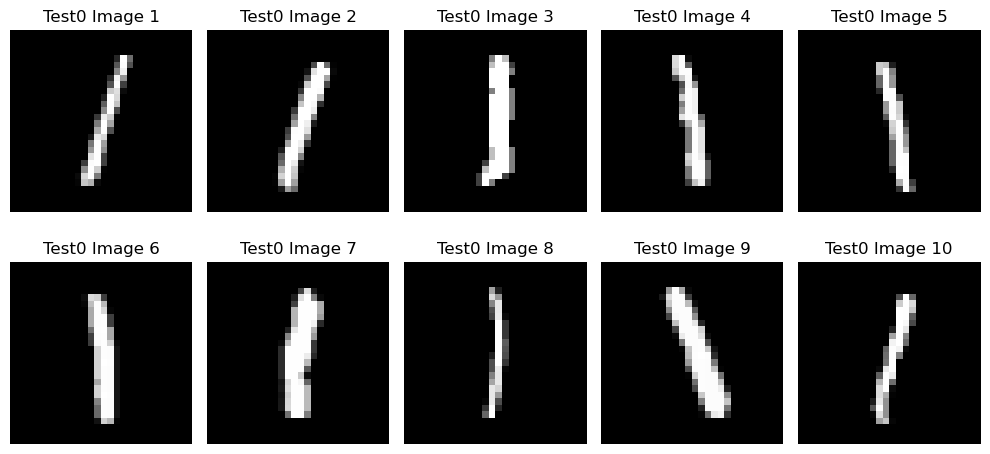
\includegraphics[width=0.7\linewidth]{files/57c9ae72ef348940f96b8b7deccd295f.png}

\subparagraph{Task 1: Extract Features and Create Dataframes}

You need to first extract features from your original trainset in order to convert the original data arrays to 2-Dimensional data points.

You are required to extract the following two features for each image:

\begin{verbatim}
● Feature1: The average brightness of each image (average all pixel brightness values within a whole image array)
                                                  
● Feature2: The standard deviation of the brightness of each image (standard deviation of all pixel brightness values within a whole image array)
\end{verbatim}

We assume that these two features are independent and that each image is drawn from a normal distribution.

\subparagraph{Train0}

\begin{verbatim}
train0_brightness_means_list = []
train0_brightness_var_list   = []
train0_brightness_stds_list  = []

for image in train0:
    train0_brightness_means_list.append(np.mean(image))
    train0_brightness_var_list.append(np.var(image))
    train0_brightness_stds_list.append(np.std(image))
\end{verbatim}

\begin{verbatim}
train0_features_df = pd.DataFrame({
    'Mean_Brightness': train0_brightness_means_list,
    'Var_Brightness' : train0_brightness_var_list,
    'STD_Brightness' : train0_brightness_stds_list
})
\end{verbatim}

\begin{verbatim}
train0_features_df.head(5)
\end{verbatim}

\bigskip\noindent
\begin{tabular}{p{\dimexpr 0.250\linewidth-2\tabcolsep}p{\dimexpr 0.250\linewidth-2\tabcolsep}p{\dimexpr 0.250\linewidth-2\tabcolsep}p{\dimexpr 0.250\linewidth-2\tabcolsep}}
\toprule
 & Mean\_Brightness & Var\_Brightness & STD\_Brightness \\
\hline
0 & 38.588010 & 6932.997356 & 83.264622 \\
\hline
1 & 37.227041 & 6170.402534 & 78.551910 \\
\hline
2 & 46.089286 & 8029.668048 & 89.608415 \\
\hline
3 & 52.757653 & 9140.553513 & 95.606242 \\
\hline
4 & 53.776786 & 9089.107063 & 95.336809 \\
\hline
\bottomrule
\end{tabular}

\bigskip

\subparagraph{Train1}

\begin{verbatim}
train1_brightness_means_list = []
train1_brightness_var_list   = []
train1_brightness_stds_list  = []

for image in train1:
    train1_brightness_means_list.append(np.mean(image))
    train1_brightness_var_list.append(np.var(image))
    train1_brightness_stds_list.append(np.std(image))
\end{verbatim}

\begin{verbatim}
train1_features_df = pd.DataFrame({
    'Mean_Brightness': train1_brightness_means_list,
    'Var_Brightness' : train1_brightness_var_list,
    'STD_Brightness' : train1_brightness_stds_list
})
\end{verbatim}

\begin{verbatim}
train1_features_df.head(5)
\end{verbatim}

\bigskip\noindent
\begin{tabular}{p{\dimexpr 0.250\linewidth-2\tabcolsep}p{\dimexpr 0.250\linewidth-2\tabcolsep}p{\dimexpr 0.250\linewidth-2\tabcolsep}p{\dimexpr 0.250\linewidth-2\tabcolsep}}
\toprule
 & Mean\_Brightness & Var\_Brightness & STD\_Brightness \\
\hline
0 & 26.135204 & 4828.525087 & 69.487589 \\
\hline
1 & 25.297194 & 5172.060910 & 71.917042 \\
\hline
2 & 20.318878 & 4121.806480 & 64.201297 \\
\hline
3 & 15.904337 & 3099.683451 & 55.674801 \\
\hline
4 & 18.876276 & 3804.478315 & 61.680453 \\
\hline
\bottomrule
\end{tabular}

\bigskip

\subparagraph{Test0}

\begin{verbatim}
test0_brightness_means_list = []
test0_brightness_var_list   = []
test0_brightness_stds_list  = []

for image in test0:
    test0_brightness_means_list.append(np.mean(image))
    test0_brightness_var_list.append(np.var(image))
    test0_brightness_stds_list.append(np.std(image))
\end{verbatim}

\begin{verbatim}
test0_features_df = pd.DataFrame({
    'Mean_Brightness': test0_brightness_means_list,
    'Var_Brightness' : test0_brightness_var_list,
    'STD_Brightness' : test0_brightness_stds_list
})
\end{verbatim}

\begin{verbatim}
test0_features_df.head(5)
\end{verbatim}

\bigskip\noindent
\begin{tabular}{p{\dimexpr 0.250\linewidth-2\tabcolsep}p{\dimexpr 0.250\linewidth-2\tabcolsep}p{\dimexpr 0.250\linewidth-2\tabcolsep}p{\dimexpr 0.250\linewidth-2\tabcolsep}}
\toprule
 & Mean\_Brightness & Var\_Brightness & STD\_Brightness \\
\hline
0 & 47.211735 & 8538.503638 & 92.404024 \\
\hline
1 & 37.960459 & 6664.361957 & 81.635543 \\
\hline
2 & 37.508929 & 6705.413186 & 81.886587 \\
\hline
3 & 67.417092 & 11160.393636 & 105.642764 \\
\hline
4 & 43.903061 & 7902.750807 & 88.897417 \\
\hline
\bottomrule
\end{tabular}

\bigskip

\subparagraph{Test1}

\begin{verbatim}
test1_brightness_means_list = []
test1_brightness_var_list   = []
test1_brightness_stds_list  = []

for image in test1:
    test1_brightness_means_list.append(np.mean(image))
    test1_brightness_var_list.append(np.var(image))
    test1_brightness_stds_list.append(np.std(image))
\end{verbatim}

\begin{verbatim}
test1_features_df = pd.DataFrame({
    'Mean_Brightness': test1_brightness_means_list,
    'Var_Brightness' : test1_brightness_var_list,
    'STD_Brightness' : test1_brightness_stds_list
})
\end{verbatim}

\begin{verbatim}
test1_features_df.head(5)
\end{verbatim}

\bigskip\noindent
\begin{tabular}{p{\dimexpr 0.250\linewidth-2\tabcolsep}p{\dimexpr 0.250\linewidth-2\tabcolsep}p{\dimexpr 0.250\linewidth-2\tabcolsep}p{\dimexpr 0.250\linewidth-2\tabcolsep}}
\toprule
 & Mean\_Brightness & Var\_Brightness & STD\_Brightness \\
\hline
0 & 12.590561 & 2387.943329 & 48.866587 \\
\hline
1 & 17.672194 & 3542.103002 & 59.515569 \\
\hline
2 & 20.661990 & 4416.420188 & 66.456152 \\
\hline
3 & 16.311224 & 3271.737323 & 57.199102 \\
\hline
4 & 13.803571 & 2739.132334 & 52.336721 \\
\hline
\bottomrule
\end{tabular}

\bigskip

\subparagraph{Task 2: Calculate Parameters}

You need to calculate all the parameters for the two-class naive bayes classifiers respectively, based upon the 2-D data points you generated in Task 1 (In total, you should have 8 parameters).

\begin{verbatim}
● Feature1: The average brightness of each image (average all pixel brightness values within a whole image array)
                                                  
● Feature2: The standard deviation of the brightness of each image (standard deviation of all pixel brightness values within a whole image array)

● (No.1) Mean of feature1 for digit0

● (No.2) Variance of feature1 for digit0

● (No.3) Mean of feature2 for digit0

● (No.4) Variance of feature2 for digit0

● (No.5) Mean of feature1 for digit1

● (No.6) Variance of feature1 for digit1

● (No.7) Mean of feature2 for digit1

● (No.8) Variance of feature2 for digit1
\end{verbatim}

\subparagraph{(Number 1) Mean of Feature 1 for Digit0}

\begin{verbatim}
mean_of_feature_1_for_digit_0 = \
    train0_features_df['Mean_Brightness'].mean()
mean_of_feature_1_for_digit_0
\end{verbatim}

\begin{verbatim}
44.12499566326531
\end{verbatim}

\subparagraph{(Number 2) Variance of Feature 1 for Digit0}

\begin{verbatim}
var_of_feature_1_for_digit_0 = \
    train0_features_df['Mean_Brightness'].var()
var_of_feature_1_for_digit_0
\end{verbatim}

\begin{verbatim}
113.87866573241182
\end{verbatim}

\subparagraph{(Number 3) Mean of Feature 2 for Digit0}

\begin{verbatim}
mean_of_feature_2_for_digit_0 = \
    train0_features_df['STD_Brightness'].mean()
mean_of_feature_2_for_digit_0
\end{verbatim}

\begin{verbatim}
87.36115347709882
\end{verbatim}

\subparagraph{(Number 4) Variance of Feature 2 for Digit0}

\begin{verbatim}
var_of_feature_2_for_digit_0 = \
    train0_features_df['STD_Brightness'].var()
var_of_feature_2_for_digit_0
\end{verbatim}

\begin{verbatim}
100.60494343865591
\end{verbatim}

\subparagraph{(Number 5) Mean of Feature 1 for Digit1}

\begin{verbatim}
mean_of_feature_1_for_digit_1 = \
    train1_features_df['Mean_Brightness'].mean()
mean_of_feature_1_for_digit_1
\end{verbatim}

\begin{verbatim}
19.33574387755102
\end{verbatim}

\subparagraph{(Number 6) Variance of Feature 1 for Digit1}

\begin{verbatim}
var_of_feature_1_for_digit_1 = \
    train1_features_df['Mean_Brightness'].var()
var_of_feature_1_for_digit_1
\end{verbatim}

\begin{verbatim}
31.102708904998412
\end{verbatim}

\subparagraph{(Number 7) Mean of Feature 2 for Digit1}

\begin{verbatim}
mean_of_feature_2_for_digit_1 = \
    train1_features_df['STD_Brightness'].mean()
mean_of_feature_2_for_digit_1
\end{verbatim}

\begin{verbatim}
61.3021791021863
\end{verbatim}

\subparagraph{(Number 8) Variance of Feature 2 for Digit1}

\begin{verbatim}
var_of_feature_2_for_digit_1 = \
    train1_features_df['STD_Brightness'].var()
var_of_feature_2_for_digit_1
\end{verbatim}

\begin{verbatim}
82.06104282975468
\end{verbatim}

\subparagraph{Implement Naive Bayes Classifier}

\subparagraph{Probability Class 0}

\begin{verbatim}
test0_features_df['Prob_Class0'] = \
    (
        norm.pdf(test0_features_df['Mean_Brightness'],
                 loc=mean_of_feature_1_for_digit_0,
                 scale=np.sqrt(var_of_feature_1_for_digit_0)
        ) * \

        norm.pdf(test0_features_df['STD_Brightness'],
                 loc=mean_of_feature_2_for_digit_0,
                 scale=np.sqrt(var_of_feature_2_for_digit_0)
        ) * \
        0.5 # Prior probability
    )
\end{verbatim}

\begin{verbatim}
test0_features_df.head(5)
\end{verbatim}

\bigskip\noindent
\begin{tabular}{p{\dimexpr 0.125\linewidth-2\tabcolsep}p{\dimexpr 0.125\linewidth-2\tabcolsep}p{\dimexpr 0.125\linewidth-2\tabcolsep}p{\dimexpr 0.125\linewidth-2\tabcolsep}p{\dimexpr 0.125\linewidth-2\tabcolsep}p{\dimexpr 0.125\linewidth-2\tabcolsep}p{\dimexpr 0.125\linewidth-2\tabcolsep}p{\dimexpr 0.125\linewidth-2\tabcolsep}}
\toprule
 & Mean\_Brightness & Var\_Brightness & STD\_Brightness & Prob\_Class0 & Prob\_Class1 & Predicted Label & Ground\_Truth\_Label \\
\hline
0 & 47.211735 & 8538.503638 & 92.404024 & 0.000628 & 1.630825e-11 & 0 & 0 \\
\hline
1 & 37.960459 & 6664.361957 & 81.635543 & 0.000535 & 4.802774e-07 & 0 & 0 \\
\hline
2 & 37.508929 & 6705.413186 & 81.886587 & 0.000529 & 5.892676e-07 & 0 & 0 \\
\hline
3 & 67.417092 & 11160.393636 & 105.642764 & 0.000013 & 7.153347e-25 & 0 & 0 \\
\hline
4 & 43.903061 & 7902.750807 & 88.897417 & 0.000735 & 9.300289e-10 & 0 & 0 \\
\hline
\bottomrule
\end{tabular}

\bigskip

\begin{verbatim}
test0_features_df['Prob_Class1'] = \
    (
        norm.pdf(test0_features_df['Mean_Brightness'],
                loc=mean_of_feature_1_for_digit_1,
                scale=np.sqrt(var_of_feature_1_for_digit_1)
        ) * \

        norm.pdf(test0_features_df['STD_Brightness'],
                loc=mean_of_feature_2_for_digit_1,
                scale=np.sqrt(var_of_feature_2_for_digit_1)
        ) * \
        0.5 # Prior probability
    )
\end{verbatim}

\begin{verbatim}
#test0_features_df.head()
\end{verbatim}

\begin{verbatim}
test0_features_df['Predicted Label'] = \
    np.where(
        test0_features_df['Prob_Class0'] > test0_features_df['Prob_Class1'], 0, 1
    )
\end{verbatim}

\begin{verbatim}
#test0_features_df.head(20)
\end{verbatim}

\subparagraph{Visualize Classification Results for Class 0}

\begin{verbatim}
# Extract index and predicted labels
indices = test0_features_df.index
predicted_labels = test0_features_df['Predicted Label']

# Create a scatter plot
plt.figure(figsize=(10, 6))
plt.scatter(indices, predicted_labels, c=predicted_labels, cmap='viridis', edgecolor='k')
plt.title("Predicted Labels vs. Image Index", fontsize=14)
plt.xlabel("Image Index", fontsize=12)
plt.ylabel("Predicted Label", fontsize=12)
plt.yticks([0, 1], labels=["Class 0", "Class 1"])
plt.grid(alpha=0.3)
plt.show()
\end{verbatim}

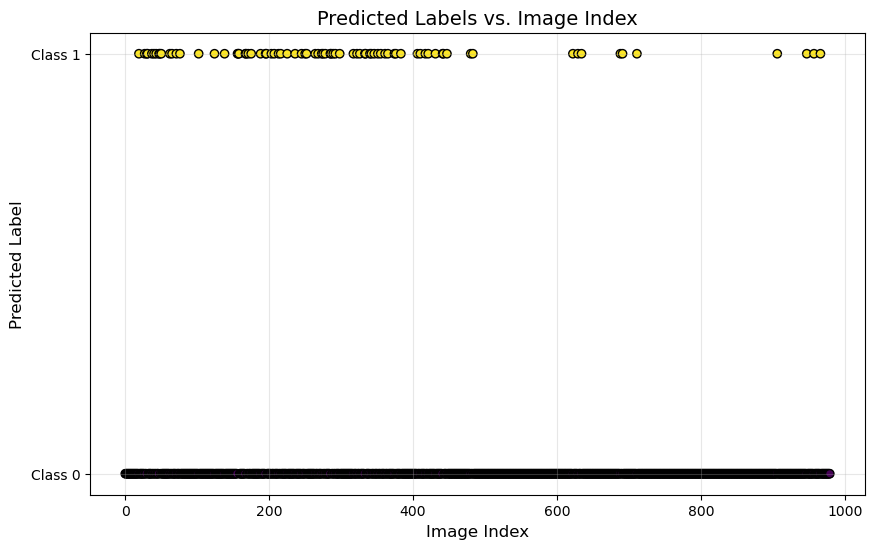
\includegraphics[width=0.7\linewidth]{files/ae26ab5986aec0dc3dceb59d48d1178c.png}

\begin{verbatim}
# Aggregate the counts of Class 0 and Class 1
class_counts = test0_features_df['Predicted Label'].value_counts()

# Create a bar chart
plt.figure(figsize=(8, 5))
plt.bar(class_counts.index, class_counts.values, color=['blue', 'orange'], alpha=0.7)
plt.title("Aggregate Counts of Predicted Labels For Test Class 0", fontsize=14)
plt.xlabel("Predicted Label", fontsize=12)
plt.ylabel("Count", fontsize=12)
plt.xticks([0, 1], labels=["Class 0", "Class 1"])
plt.grid(axis='y', alpha=0.3)

# Annotate counts on top of bars
for i, count in enumerate(class_counts.values):
    plt.text(i, count + 5, str(count), ha='center', fontsize=12)

plt.show()
\end{verbatim}

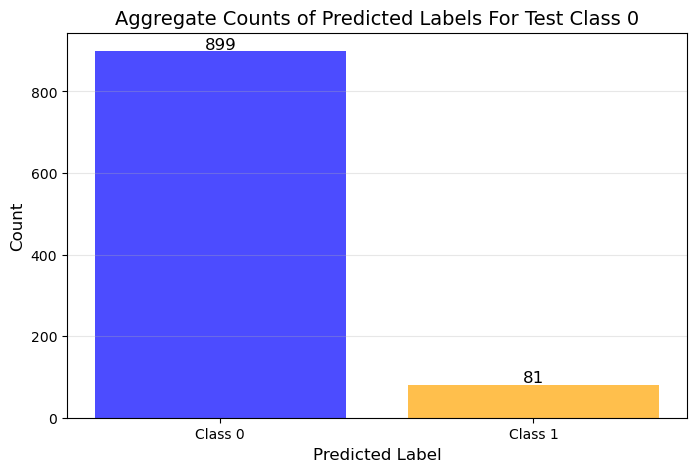
\includegraphics[width=0.7\linewidth]{files/730d6f351d16851d7b1ad533cbde8f77.png}

\begin{verbatim}
# Extract the data
indices = test0_features_df.index
prob_class0 = test0_features_df['Prob_Class0']
prob_class1 = test0_features_df['Prob_Class1']

# Scatter plot for Prob_Class0
plt.figure(figsize=(12, 6))
plt.scatter(indices, prob_class0, color='blue', label='Prob_Class0', alpha=0.7, edgecolor='k')

# Scatter plot for Prob_Class1
plt.scatter(indices, prob_class1, color='orange', label='Prob_Class1', alpha=0.7, edgecolor='k')

# Add labels and legend
plt.title("Scatter Plot of Probabilities for Class 0 and Class 1", fontsize=14)
plt.xlabel("Image Index", fontsize=12)
plt.ylabel("Probability", fontsize=12)
plt.legend(fontsize=12)
plt.grid(alpha=0.3)
plt.show()
\end{verbatim}

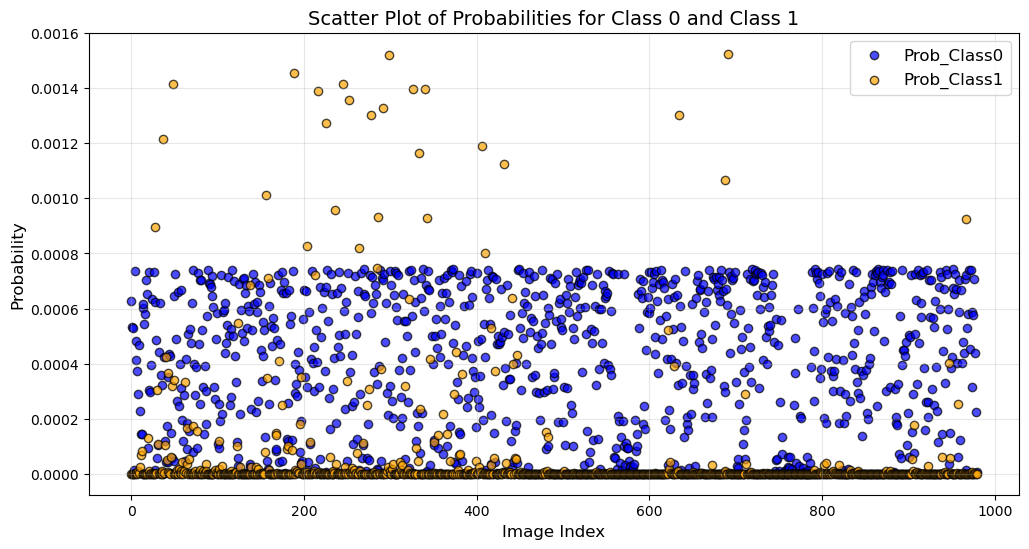
\includegraphics[width=0.7\linewidth]{files/d1dce019cc94fd6b8b3da8f45d219320.png}

\subparagraph{Probability Class 1}

\begin{verbatim}
test1_features_df['Prob_Class0'] = \
    (
        norm.pdf(test1_features_df['Mean_Brightness'],
                 loc=mean_of_feature_1_for_digit_0,
                 scale=np.sqrt(var_of_feature_1_for_digit_0)
        ) * \

        norm.pdf(test1_features_df['STD_Brightness'],
                 loc=mean_of_feature_2_for_digit_0,
                 scale=np.sqrt(var_of_feature_2_for_digit_0)
        ) * \
        0.5 # Prior probability
    )
\end{verbatim}

\begin{verbatim}
#test1_features_df.head(10)
\end{verbatim}

\begin{verbatim}
test1_features_df['Prob_Class1'] = \
    (
        norm.pdf(test1_features_df['Mean_Brightness'],
                loc=mean_of_feature_1_for_digit_1,
                scale=np.sqrt(var_of_feature_1_for_digit_1)
        ) * \

        norm.pdf(test1_features_df['STD_Brightness'],
                loc=mean_of_feature_2_for_digit_1,
                scale=np.sqrt(var_of_feature_2_for_digit_1)
        ) * \
        0.5 # Prior probability
    )
\end{verbatim}

\begin{verbatim}
#test1_features_df.head()
\end{verbatim}

\begin{verbatim}
test1_features_df['Predicted Label'] = \
    np.where(
        test1_features_df['Prob_Class0'] > test1_features_df['Prob_Class1'], 0, 1
    )
\end{verbatim}

\begin{verbatim}
#test1_features_df.head(20)
\end{verbatim}

\subparagraph{Visualize Classification Results for Class 1}

\begin{verbatim}
# Extract index and predicted labels
indices = test1_features_df.index
predicted_labels = test1_features_df['Predicted Label']

# Create a scatter plot
plt.figure(figsize=(10, 6))
plt.scatter(indices, predicted_labels, c=predicted_labels, cmap='viridis', edgecolor='k')
plt.title("Predicted Labels vs. Image Index", fontsize=14)
plt.xlabel("Image Index", fontsize=12)
plt.ylabel("Predicted Label", fontsize=12)
plt.yticks([0, 1], labels=["Class 0", "Class 1"])
plt.grid(alpha=0.3)
plt.show()
\end{verbatim}

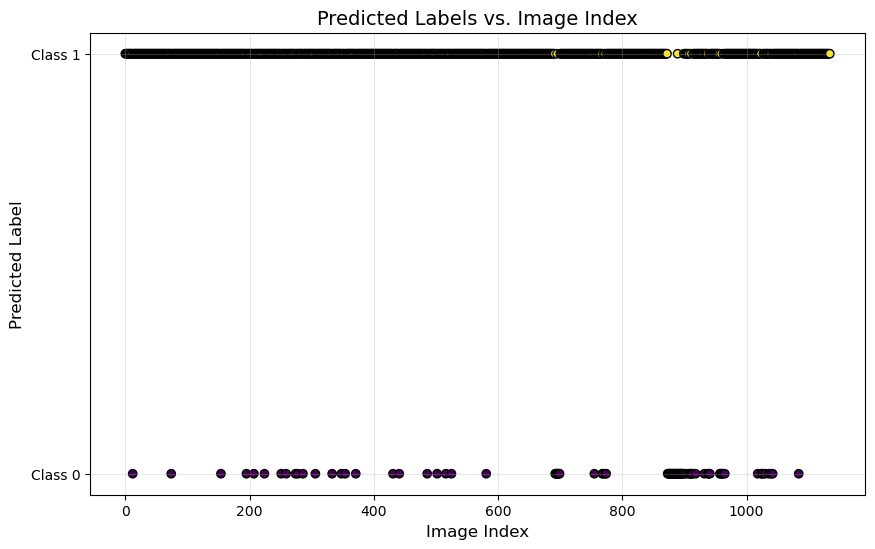
\includegraphics[width=0.7\linewidth]{files/6b5754c4812731e49f8e7091890bc960.png}

\begin{verbatim}
# Aggregate the counts of Class 0 and Class 1
class_counts = test1_features_df['Predicted Label'].value_counts()

# Sort the counts by label to ensure consistent order (0, 1)
class_counts = class_counts.sort_index()

# Create a bar chart
plt.figure(figsize=(8, 5))
plt.bar(class_counts.index, class_counts.values, color=['blue', 'orange'], alpha=0.7)
plt.title("Aggregate Counts of Predicted Labels for Test Class 1", fontsize=14)
plt.xlabel("Predicted Label", fontsize=12)
plt.ylabel("Count", fontsize=12)
plt.xticks([0, 1], labels=["Class 0", "Class 1"])
plt.grid(axis='y', alpha=0.3)

# Annotate counts on top of bars
for i, count in enumerate(class_counts.values):
    plt.text(i, count + 5, str(count), ha='center', fontsize=12)

plt.show()
\end{verbatim}

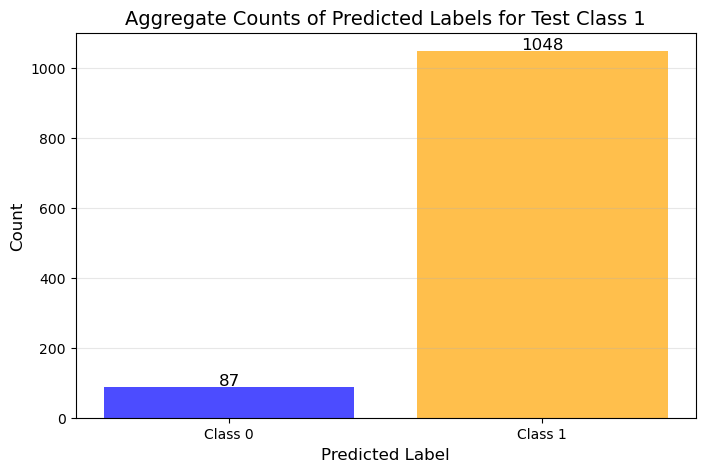
\includegraphics[width=0.7\linewidth]{files/e0a463be9998c62f4e65ea7aba7d92a0.png}

\begin{verbatim}
# Extract the data
indices = test1_features_df.index
prob_class0 = test1_features_df['Prob_Class0']
prob_class1 = test1_features_df['Prob_Class1']

# Scatter plot for Prob_Class0
plt.figure(figsize=(12, 6))
plt.scatter(indices, prob_class0, color='blue', label='Prob_Class0', alpha=0.7, edgecolor='k')

# Scatter plot for Prob_Class1
plt.scatter(indices, prob_class1, color='orange', label='Prob_Class1', alpha=0.7, edgecolor='k')

# Add labels and legend
plt.title("Scatter Plot of Probabilities for Class 0 and Class 1", fontsize=14)
plt.xlabel("Image Index", fontsize=12)
plt.ylabel("Probability", fontsize=12)
plt.legend(fontsize=12)
plt.grid(alpha=0.3)
plt.show()
\end{verbatim}

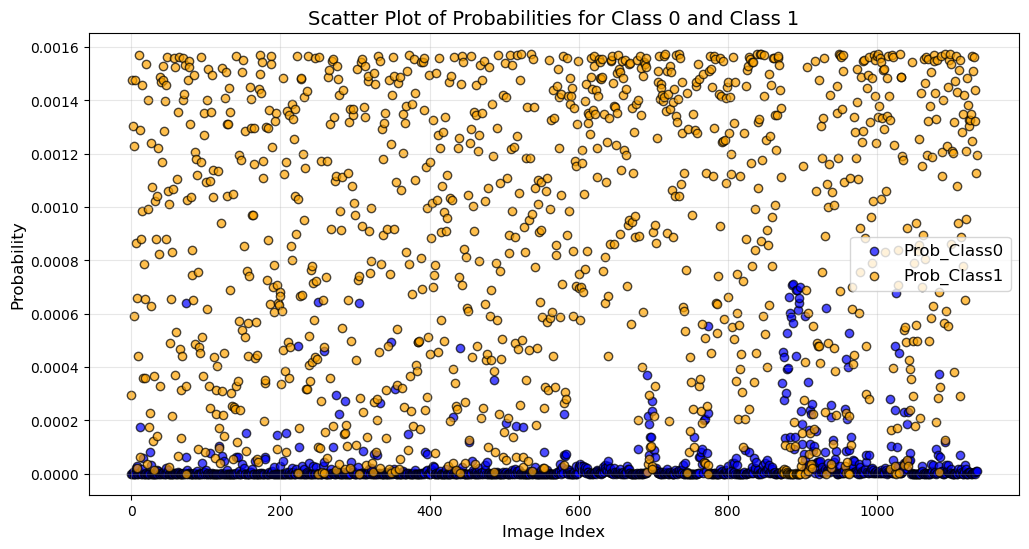
\includegraphics[width=0.7\linewidth]{files/391b9bd75bc54f24055c9121b1afefb7.png}

\subparagraph{Accuracy Calculations}

\subparagraph{Create Ground Truth Labels}

\begin{verbatim}
test0_features_df['Ground_Truth_Label'] = 0
test1_features_df['Ground_Truth_Label'] = 1
\end{verbatim}

\begin{verbatim}
#test0_features_df.head(20)
\end{verbatim}

\begin{verbatim}
#test1_features_df.head(20)
\end{verbatim}

\subparagraph{Calculate Accuracy for Class 0}

\begin{verbatim}
accuracy_class0 = \
    accuracy_score(
        test0_features_df['Ground_Truth_Label'],
        test0_features_df['Predicted Label']
    )
print(f"Accuracy for Class 0: {accuracy_class0 * 100:.2f}%")
\end{verbatim}

\begin{verbatim}
Accuracy for Class 0: 91.73%
\end{verbatim}

\begin{verbatim}
# Generate confusion matrix
conf_matrix_class_0 = \
    confusion_matrix(
        test0_features_df['Ground_Truth_Label'],
        test0_features_df['Predicted Label']
    )
conf_matrix_class_0
\end{verbatim}

\begin{verbatim}
array([[899,  81],
       [  0,   0]])
\end{verbatim}

\subparagraph{Display Confusion Matrix for Class 0}

\begin{verbatim}
# Visualize confusion matrix
plt.figure(figsize=(8, 6))
sns.heatmap(conf_matrix_class_0, annot=True, fmt='d', cmap='Blues', xticklabels=["Class 0", "Class 1"], yticklabels=["Class 0", "Class 1"])
plt.title("Confusion Matrix", fontsize=14)
plt.xlabel("Predicted Label", fontsize=12)
plt.ylabel("Actual Label", fontsize=12)
plt.show()
\end{verbatim}

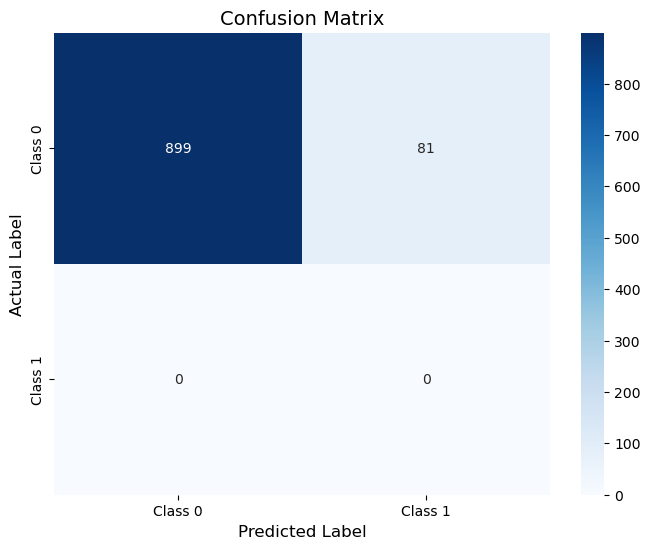
\includegraphics[width=0.7\linewidth]{files/6ca052b0afc54d0bddd1931d6757e6bc.png}

\subparagraph{Calculate Accuracy for Class 1}

\begin{verbatim}
accuracy_class1 = \
    accuracy_score(
        test1_features_df['Ground_Truth_Label'],
        test1_features_df['Predicted Label']
    )
print(f"Accuracy for Class 1: {accuracy_class1 * 100:.2f}%")
\end{verbatim}

\begin{verbatim}
Accuracy for Class 1: 92.33%
\end{verbatim}

\begin{verbatim}
# Generate confusion matrix
conf_matrix_class_1 = \
    confusion_matrix(
        test1_features_df['Ground_Truth_Label'],
        test1_features_df['PredicteSd Label']
    )
conf_matrix_class_1
\end{verbatim}

\begin{verbatim}
array([[   0,    0],
       [  87, 1048]])
\end{verbatim}

\subparagraph{Display Confusion Matrix for Class 1}

\begin{verbatim}
# Visualize confusion matrix
plt.figure(figsize=(8, 6))
sns.heatmap(conf_matrix_class_1, annot=True, fmt='d', cmap='Blues', xticklabels=["Class 0", "Class 1"], yticklabels=["Class 0", "Class 1"])
plt.title("Confusion Matrix", fontsize=14)
plt.xlabel("Predicted Label", fontsize=12)
plt.ylabel("Actual Label", fontsize=12)
plt.show()
\end{verbatim}

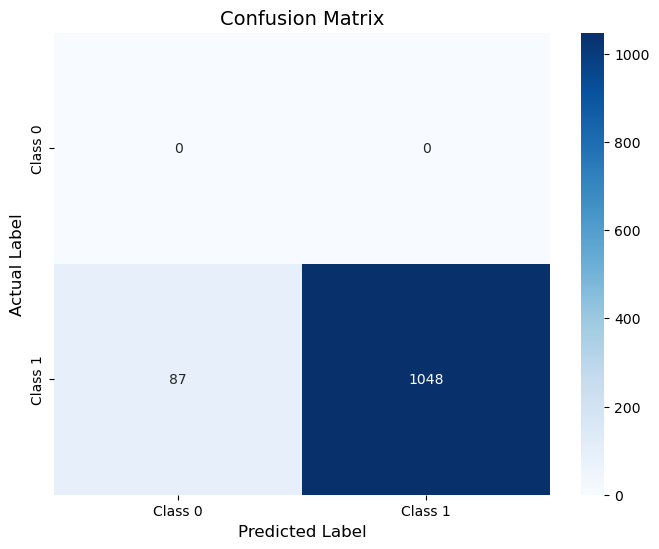
\includegraphics[width=0.7\linewidth]{files/402c53081de71531e526c4576b358f5a.png}

\subparagraph{Create Answer List}

\begin{verbatim}
answer_list = [
    myID,
    float(mean_of_feature_1_for_digit_0),
    float(var_of_feature_1_for_digit_0),
    float(mean_of_feature_2_for_digit_0),
    float(var_of_feature_2_for_digit_0),
    float(mean_of_feature_1_for_digit_1),
    float(var_of_feature_1_for_digit_1),
    float(mean_of_feature_2_for_digit_1),
    float(var_of_feature_2_for_digit_1),
    float(accuracy_class0),
    float(accuracy_class1)
]
\end{verbatim}

\begin{verbatim}
len(answer_list)
\end{verbatim}

\begin{verbatim}
11
\end{verbatim}

\begin{verbatim}
answer_list
\end{verbatim}

\begin{verbatim}
['5806',
 44.12499566326531,
 113.87866573241182,
 87.36115347709882,
 100.60494343865591,
 19.33574387755102,
 31.102708904998412,
 61.3021791021863,
 82.06104282975468,
 0.9173469387755102,
 0.9233480176211454]
\end{verbatim}